\documentclass[titlepage = firstcover]{scrartcl}
\usepackage[aux]{rerunfilecheck}
\usepackage{fontspec}
\usepackage[main=ngerman, english, french]{babel}

% mehr Pakete hier
\usepackage{expl3}
\usepackage{xparse}

%Mathematik------------------------------------------------------
\usepackage{amsmath}   % unverzichtbare Mathe-Befehle
\usepackage{amssymb}   % viele Mathe-Symbole
\usepackage{mathtools} % Erweiterungen für amsmath
\usepackage[
  math-style=ISO,    % \
  bold-style=ISO,    % |
  sans-style=italic, % | ISO-Standard folgen
  nabla=upright,     % |
  partial=upright,   % /
]{unicode-math}% "Does exactly what it says on the tin."

% Laden von OTF-Mathefonts
% Ermöglich Unicode Eingabe von Zeichen: α statt \alpha

\setmathfont{Latin Modern Math}
%\setmathfont{Tex Gyre Pagella Math} % alternativ zu Latin Modern Math
\setmathfont{XITS Math}[range={scr, bfscr}]
\setmathfont{XITS Math}[range={cal, bfcal}, StylisticSet=1]

\AtBeginDocument{ % wird bei \begin{document}
  % werden sonst wieder von unicode-math überschrieben
  \RenewDocumentCommand \Re {} {\operatorname{Re}}
  \RenewDocumentCommand \Im {} {\operatorname{Im}}
}
\usepackage{mleftright}
\setlength{\delimitershortfall}{-1sp}

%Sprache----------------------------------------------------------
\usepackage{microtype}
\usepackage{xfrac}
\usepackage[autostyle]{csquotes}    % babel
\usepackage[unicode, pdfusetitle]{hyperref}
\usepackage{bookmark}
\usepackage[shortcuts]{extdash}
%Einstellungen hier, z.B. Fonts
\usepackage{booktabs} % Tabellen

%Defininierte funktionen
\DeclareMathOperator{\f}{xyz}

\ExplSyntaxOn % bequeme Syntax für Definition von Befehlen

\NewDocumentCommand \I {} {         %Befehl \I definieren,keine Argumente
  \symup{i}                         %Ergebnis von \I
} 
\NewDocumentCommand \dif {m} % m = mandatory (Pflichtargument für \dif)
{
  \mathinner{\symup{d} #1}
}

\ExplSyntaxOff % Syntax wieder ausschalten. Wichtig!


\title{Das Trägheitsmoment}
\author{
  David Gutnikov\\
  \href{mailto:david.gutnikov@udo.edu}{david.gutnikov@udo.edu}
 \and 
  Lasse Sternemann\\
  \href{mailto:lasse.sternemann@udo.edu}{lasse.sternemann@udo.edu}
}
\date{Durchführung am 19.11.2019}

\begin{document}
    \maketitle
    \tableofcontents
    \newpage

    \section{Zielsetzung}
    Es sollen Trägheitsmomente verschiedener Körper durch Experimente gemessen und durch entsprechende Rechnungen überprüft werden. 
    Dabei wird auch der in den Rechnungen angewandte Satz von Steiner durch die Messungen bestätigt. Die verschiedenen Körper sind dabei 
    allesamt starre Symmetriekörper wie Kugeln und Zylinder oder werden als diese angenähert.

    \section{Theoretische Grundlagen}
      \subsection{Trägheitsmoment}
      Das Trägheitsmoment beschreibt das Streben einer Masse sich gegen die Änderung der Winkelgeschwindigkeit zu widersetzen. Damit stellt es 
      das Äquivalent zur trägen Masse dar, welche sich der translativen Beschleunigung entgegensetzt. So gehen in die translative kinetische Energie
      die Masse und die Geschwindigkeit ein und in die Rotationsenergie das Trägheitsmoment und die Winkelgeschwindigkeit.
      \begin{align*}
        E_{\text{trans}} = \frac{1}{2} mv^2 \\
        E_{\text{rot}} = \frac{1}{2}J \omega^2
      \end{align*}
      Standardmäßig betrachtet man das Trägheitsmoment bezüglich der Drehachse durch den Schwerpunkt des Körpers. So lässt sich das Trägheitsmoment 
      $J$ für einen Körper aus vielen homogen verteilten Massenpunkten m durch Formel 1 berechnen. Dabei bezeichnet $m$ die Masse der einzelnen 
      Massenpunkte und $r$ deren senkrechten Abstand zur Drehachse.
      \begin{equation}
        J = \sum_{i=1}^n m_i \cdot r_i^2
      \end{equation}
      Um die Berechnung auf für reelle Körper genau möglich zu machen, reduziert man die Größe der Massenpunkte bis sie infinitesimal klein werden und  
      nun anstatt aufzusummieren über sie Integrieren werden kann. Daraus ergibt sich Formel 3.
      \begin{equation}
        J = \int r^2 dm
      \end{equation}
      Da die Masse der einzelnen Massenpunkte nicht bekannt ist, werden Trägheitsmomente normalerweise berechnet, indem man die Dichteverteilung des Körpers 
      über das Volumen integriert. Bei den gemessenen Körpern liegen homogene Massenverteilungen vor, sodass sich zur Berechnung derer Trägheitsmomente 
      Formel 2 ergibt.  
      \begin{equation}
        J = \int_V r^2 \rho dV
      \end{equation}
      Das Berechnen der Allgemeinen Trägheitsmomente, der für den Versuch nötigen Körper, liefert die Formeln 4 bis 6.
      \begin{align}
        J_{Zylisym} = \frac{1}{2}mr^2 \\
        J_{Zyliquer} = m(\frac{1}{4}r^2 + \frac{1}{12}l^2) \\
        J_{Kugel} = \frac{2}{5}mr^2
      \end{align}
      \begin{figure}[h]
        \centering
        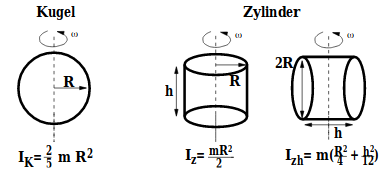
\includegraphics[width=0.7\linewidth]{TM.png}
        \caption{In der Abbildung sind die in den Formeln 4 bis 6 stehenden Trägheitsmomente ihren Körpern und Drehachsen zugeordnet. [1, S.2]}
      \end{figure}
      Das Trägheitsmoment eines homogenen  Vollzylinders, der sich um seine Symmetrieachse dreht, wird durch Formel 4 beschrieben. $m$ steht dabei für dessen
      Masse und $r$ für den Radius des Vollzylinders. Wenn der selbe Vollzylinder um seine Querachse rotiert, wird sein Trägheitsmoment durch Formel 5 beschrieben 
      und das im Vergleich zu Formel 4 neue $l$ steht für seine Länge. Der letzte Körper ist eine Kugel, die von Natur aus immer um ihre Hauptträgheitsachse 
      rotiert. Ihr Trägheitsmoment wird durch Formel 6 beschrieben, wobei $m$ für ihre Masse und $r$ für ihren Radius steht. Bei dem im Experiment vorliegenden System
      kommt es zu einer Schwingung mit der in Formel 7 beschriebenen Schwingungsdauer, über die ebenfalls das Trägheitsmoment des Körpers berechnet werden kann, wenn
      $D$ und $T$ bekannt sind.
      \begin{equation}
        T = 2\pi \sqrt{\frac{I}{D}}
      \end{equation}

      \subsection{Satz von Steiner}
      Die obrigen Formeln gelten nur für Körper, die um ihre Symmetrieachse rotieren. Körper die um eine Achse außerhalb ihrer Symmetrieachse rotieren, erfahren
      ein größeres Trägheitsmoment. Wenn die Drehachse parallel zu einer der Symmetrieachsen liegt, lässt sich der Zuwachs des Trägheitsmomentes durch den Satz 
      von Steiner beschreiben. 
      \begin{equation}
        J_{ges} = J_{sym} + ma^2
      \end{equation}
      Dabei wird das Gesamtträgheitsmoment, wie in Formel 8 zu sehen, aus dem Hauptträgheitsmoment des Körpers durch seine Symmetrieachse und dem zweiten 
      Summanden beschrieben. In diesem steht $m$ für die Masse des Körpers und $a$ für den senkrechten Abstand der Drehachse zur Symmetrieachse des
      Hauptträgheitsmomentes.

      \subsection{Winkelrichtgröße}
      Beim Anbringen einer Achse an eine Torsionsfeder und anschließendem Auslenken dieser, tritt eine Kraft auf, die als Drehmoment auf die angbrachte Achse im Abstand $r$
      wirkt. Damit lassen sich das Drehmoment (Formel 9) und die Winkelrichtgröße der Torsionsfeder gleichsetzen (Formel 10). Wenn die Kraft senkrecht zum Radius gemessen wird,
      beträgt der Sinus Eins und fällt weg.
      \begin{equation}
        \vec{M} = \vec{r} \times \vec{F}
      \end{equation}
      \begin{equation}
        r \cdot F \cdot \sin(\alpha) = D \cdot \upvarphi
      \end{equation}
      \begin{equation*}
        M \cdot F = D \cdot \upvarphi
      \end{equation*} 
    
    \section{Versuchsaufbau}
      Das für den Versuch grundlegende System besteht aus einer Torsionsfeder, auf der eine Drillachse befestigt ist. Auf dieser Drillachse werden für die Versuche
      verschiedene Körper oder Querachsen auf die Drillachse gesetzt. Sie sind dann so mit der Torsionsfeder verbunden, dass sie die Feder bei eigener Auslenkung auch
      auslenken. Wenn die äußere Kraft, die der Auslenkung zu Grunde liegt, wegfällt, beginnt das gesamte System des Testkörpers, der Drillachse und der 
      Torsionsfeder zu schwingen und die Schwingungsparameter können über das Messen der Schwingungsdauer bestimmt werden.
      \newpage
      \begin{figure}[h]
        \centering
        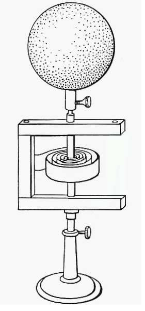
\includegraphics[width=0.3\linewidth, height=0.5\linewidth]{Versuchsaufbau.png}
        \caption{Hier ist das System mit einer Kugel als Testkörper zu sehen. Diese ist wie zuvor beschrieben so an der Drillachse befestigt, dass ihr Haupträgheitsmoment auf der Drehachse des Systems liegt. [1, S.3]}
      \end{figure}

    \section{Versuchsdurchführung}
      \subsection{Bestimmung der Apperatparameter}
      Um die späteren Versuche mit Berechnungen zu überprüfen, müssen zuerst die Apperatparameter bestimmt werden. Eines dieser Parameter ist die Winkelrichtgröße 
      der Torsionsfeder. Diese lässt sich berechnen, indem eine Achse senkrecht auf die Achse der Torsionsfeder gesetzt wird und diese dann um einen Winkel
      ausgelenkt wird. Ein Kraftmesser misst die senkrecht auf die Achse wirkende Kraft bei konstantem Abstand zur Drehachse und variierendem Auslenkwinkel. Die 
      Winkelrichtgröße lässt sich dann durch Umstellen von Formel 10 berechnen. Der zweite Parameter ist das Drehmoment der Drillachse, welches sich über 
      die Bestimmungen verschiedener Trägheitsmomente unter Zuhilfenahme des Satzes von Steiner messen lässt. Dazu werden zwei Gewichte pro Messung um weitere 2,5 cm von 
      der  Drillachse entfernt, befestigt und die Schwingungsdauer des Systems bei diesen verschieden Abständen gemessen.

      \subsection{Trägheitsmoment verschiedener Symmetriekörper}
      Zuerst wird eine homogene Holzkugel, welche unendlich viele, gleiche Trägheitsachsen hat, auf die Drillachse gesetzt und ausgelenkt. Daraufhin werden die 
      zur auftretenden Schwingung gehörigen Schwingungsdauern gemessen, um später mit jener und den Apperatparametern das Trägheitsmoment der Kugel zu bestimmen.
      Das zweite Trägheitsmoment ist das eines homogen gefüllten Zylinders bezüglich seiner Symmetrieachse. Auch hier wird das System aus Zylinder und Torsionsfeder
      ausgelenkt und die Schwingungsdauer gemessen.

      \subsection{Trägheitsmomente einer Holzpuppe}
      Es werden zwei verschiedenen Trägheitsmomente bestimmt, indem die Puppe in zwei verschiedenen Positionen auf die Drillachse gesetzt wird und dann die verschiedenen
      Schwingungsdauern des Systems gemessen werden.. In der ersten Position steht die Puppe senkrecht und hat die Arme angelegt. In der zweiten Position steht sie wieder 
      senkrecht, aber streckt die Arme nun rechtwinklig aus, sodass eine Art T-Pose entsteht. Zur späteren Verifizierung der Messergebnisse werden Kopf, Beine, Arme
      und Torso als Kugel oder Zylinder angenähert und der Satz von Steiner unter der Annahme verwendet, dass die Drehachse durch die gedachte Symmetrieachse der
      Puppe führt.

      \begin{figure}[h]
        \centering
        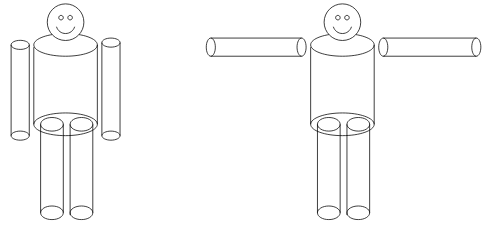
\includegraphics[width=0.7\linewidth]{Puppe.png}
        \caption{Die linke Puppe befindet sich in Position a und die rechte in Position b. [1, S.4]}
      \end{figure}

    \section{Ergebnisse und Auswertung}

      \subsection{Gerätparameter}
      \begin{table}[h]
        \centering
        \caption{$\varphi$ ist der Winkel, um den die auf der Torsionsfeder liegende Achse ausgelenkt wird und $F$ ist die Kraft, die bei zugehörigem Winkel senkrecht auf die Achse im Abstand von 20 cm zur Drehachse wirkt.}
        \label{tab:Tabelle_1}

        \begin{tabular}{c c}
          \toprule
          {$\varphi$ [°]} & {$F$ [N]} \\
          \midrule
          30 & 0,041 \\
          60 & 0,122 \\
          90 & 0,194 \\
          120 & 0,26 \\
          150 & 0,33 \\
          180 & 0,40 \\
          210 & 0,45 \\
          240 & 0,55 \\
          270 & 0,60 \\
          300 & 0,67 \\
          \bottomrule
        \end{tabular}
      \end{table}
      
      Die Winkelrichtgröße lässt sich bestimmen, indem Formel 10 nach D umgestellt wird und $\alpha$ gleich 90 Grad gesetzt wird. Nun wird für jedes Wertepaar die
      Winkelrichtgröße und daraus der Mittelwert mit zugehörigen Standardabweichung des Mittelwerts bestimmt. Dies führt zu Gleichung 11 für die gemittelte Winkelrichtgröße.

      \begin{equation*}
        \overline{D} = \sum_{i=1}^{10} (\frac{MF_i}{\upvarphi}) \cdot \frac{1}{10}
      \end{equation*}

      \begin{equation}
        \overline{D} = \overline{D} \pm \sqrt{\frac{\sum_{i=1}^{10}(D_i - \overline{D}^2)}{n(n-1)}}
      \end{equation}

      Somit ergibt sich $D$ = (0,024 $\pm$ 0,001) N .
      %\newpage
      \begin{table}[h]
        \centering
        \caption{a ist der Abstand der Gewichte von der Drehachse und T die Schwingungsdauer des Systems bei entsprechendem Abstand. Mit diesen Werten und dem Satz von Steiner lässt sich das Trägheitsmoment der Drillachse berechnen.}
        \label{tab:Tabelle_2}
        
        \begin{tabular}{c c}
          \toprule
          {$a$ [m]} & {$T$ [s]} \\
          \midrule
          0,05060 & 2,76 \\
          0,07500 & 3,16 \\
          0,10600 & 3,44 \\
          0,12500 & 3,96 \\
          0,14970 & 4,66 \\
          0,17500 & 5,02 \\
          0,20045 & 5,76 \\
          0,22500 & 6,56 \\
          0,25070 & 7,04 \\
          0,27500 & 7,69 \\
          \bottomrule
        \end{tabular}
      \end{table}
      
      Zum Bestimmen des Trägheitsmomentes der Drillachse wird $T^2$ gegen $a^2$ aufgetragen und eine lineare Regression durchgeführt, die zusammen mit den Messwerten
      in Abbildung 4 zu sehen ist. \newline

      \begin{figure}[h]
        \centering
        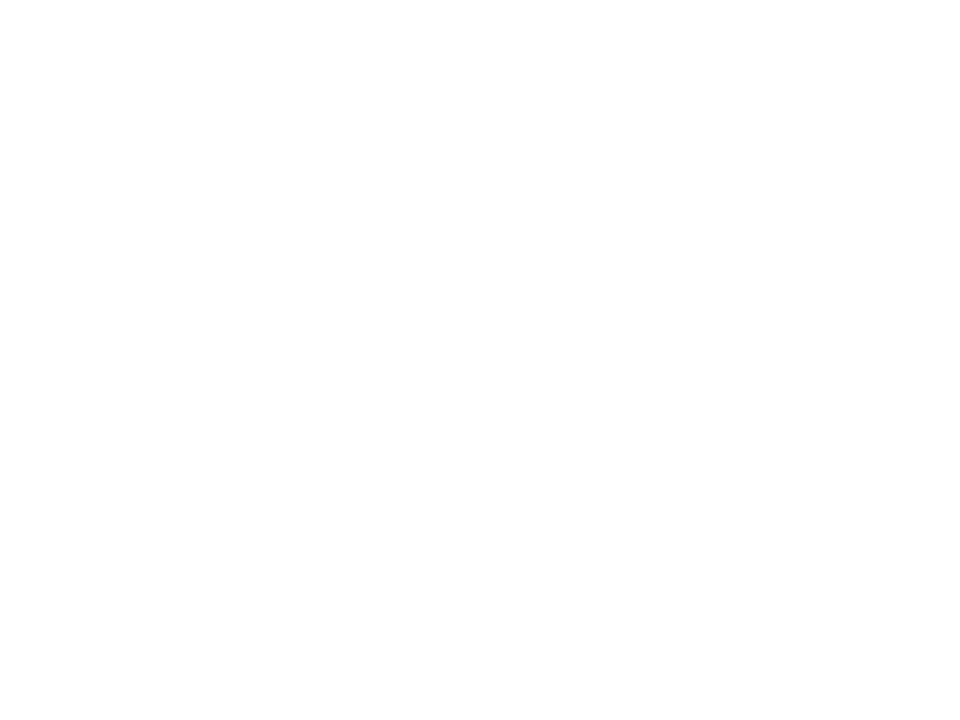
\includegraphics[width=0.8\linewidth]{Drill.pdf}
        \caption{Bei Veränderung des Abstandes a wurden immer wieder die entsprechenden T gemessen. Nun werden die Werte quadriert und T² gegen a² aufgetragen. Die gelbe Ausgleichsgerade stammt aus einer linearen Regression. Deren Steigung ist 715,169 und der y-Achsenabschnitt beträgt 5,00.}
      \end{figure}
      
      Das Gesamtträgheitsmoment $I$ setzt sich aus dem Eigenträgheitsmoment der Drehachse $I_D$ und den Trägheitsmomenten der beiden Zylinder auf der Querachse 
      $I_k$ zusammen. Die zugehörige Formel wird nach $I_D$ umgestellt.
      \begin{align*}
        I &= I_D + 2 \cdot I_k \\
        I_D &= I -2 \cdot I_k
      \end{align*}
      Dabei setzt sich $I_k$ aus dem Hauptträgheitsmoment der Zylinder und einer zusätzlichen Komponente aufgrund der Entfernung zur Drehachse zusammen.
      Anwenden des Satzes von Steiner und Einsetzen der Trägheitsmomente aus Formel 5 führen zu Formel 12.
      \begin{equation}
        I_k = I_S + ma^2 \Rightarrow I_k = m \cdot (\frac{r^2}{4} + \frac{h^2}{12}) + ma^2
      \end{equation}
      Mit dem über die Schwingungsdauer bestimmten Gesamtträgheitsmoment des Systems folgt für $I_D$:
      \begin{equation}
        I_D = \frac{D}{4\pi^2} \cdot T^2 - 2m \cdot (\frac{r^2}{4} + \frac{h^2}{12}) - 2 \cdot ma^2
      \end{equation}
      Wenn Formel 13 dann nach $T^2$ umgestellt wird, stellt dies die Geradengleichung der linearen Regression dar.
      \begin{align}
        T^2 &= \frac{8\pi^2m}{D} \cdot a^2  + \frac{4\pi^2}{D}(I_D + 2 \cdot I_S) \\
        T^2 &= m \cdot a^2 + b
      \end{align}
      Über den y-Achsenabschnitt lässt sich nun das Eigenträgheitsmoment der Drillachse mit Formel 14 bestimmen, wobei die Steigung $m = 715,17$ und der y-Achsenabschnitt $T_0^2$=5,00 ist.
      Formel 15 stellt die Geradengleichung exemplarisch dar.
      \begin{equation*}
        I_D = \frac{T_0^2D}{4\pi^2} - 2 \cdot I_S = (30 \pm 4) \cdot 10^{-4}kgm^2
      \end{equation*}
      

      \subsection{Trägheitsmomente verschiedener Körper}
      
     
      
      \begin{table}[h]
        \centering
        \caption{In der Tabelle sind die Messungen der Schwingungsdauern der Schwingungen aufgetragen, die nach dem Auslenken des Systems entstehen. Sie werden benötigt um die Trägheitsmomente zu berechnen}
        \label{tab:Tabelle_3}

        \begin{tabular}{c c}
          \toprule
          {$T_{Zyli}$ [s]} & {$T_{Kugel}$ [s]} \\
          \midrule
          0,97 & 1,69 \\
          0,83 & 1,83 \\
          0,86 & 1,80 \\
          0,92 & 1,80 \\
          0,92 & 1,72 \\
          \bottomrule
        \end{tabular}
      \end{table}
      
      Das theoretisch berechnete Trägheitsmoment des Zylinders mit einer Masse von 1,1195 kg und einem Radius von 0,035 m beträgt nach Formel 7 
      $I_{Zyli} = 6,68 \cdot 10^{-4} kgm^2$. \newline
      
      Das Trägheitsmoment des Zylinders lässt sich bestimmen, indem von dem über Formel 7 berechneten Trägheitsmoment das der Drillachse abgezogen wird. Kombiniert
      mit der Gauß`schen Fehlerfortpflanzung 
      
      \begin{equation*}
        \Delta f = \sqrt{\sum_{i=1}^N (\frac{df}{dy_i}\cdot \Delta y_i)^2}
      \end{equation*}

      bei der $\Delta f$ für den wahrscheinlichsten Fehler der abhängigen Größe steht, $N$ für die Anzahl der einfließenden, fehlerbehafteten Größen und 
      $y_i$ bzw. $\Delta y_i$ für die fehlerbehaftete Größe und deren Fehler, ergibt sich für das gemessene Trägheitsmoment folgende Formel.
      \begin{equation*}
        I_{Zyli} = \frac{D\overline{T}^2}{4\pi^2} \pm \sqrt{(\frac{D\overline{T}}{2\cdot \pi^2} \cdot \Delta \overline{T})^2 + (\frac{\overline{T}^2}{4 \cdot \pi^2} \cdot \Delta \overline{D})^2} - I_D \pm \Delta I_D
      \end{equation*}
      $I_{Zyli} = (-25 \pm 4) \cdot 10^{-4} \, kgm²$ \newline

      Das Trägheitsmoment der Kugel, der Masse 1,0376 kg und des Radius` 0,0725 m hat nach Formel 7 das Trägheitsmoment $I_{Kugel} = 1,92 \cdot 10^{-3} kgm^2$. \newline

      Experimentell lässt sich dieses Trägheitsmoment analog zu dem des Zylinders bestimmen. Hier wird das Trägheitsmoment der Drillachse vom Trägheitsmoment
      aus Formel 7 abgezogen.
      \begin{equation*}
        I_{Kugel} = \frac{D\overline{T}^2}{4\pi^2} \pm \sqrt{(\frac{D\overline{T}}{2\cdot \pi^2} \cdot \Delta \overline{T})^2 + (\frac{\overline{T}^2}{4 \cdot \pi^2} \cdot \Delta \overline{D})^2} - I_D \pm \Delta I_D
      \end{equation*}
      $I_{Kugel} = (-11 \pm 5) \cdot 10^{-4} \, kgm²$
      


      \subsection{Trägheitsmomente der Holzpuppe}

      
      Zum Bestimmen der Trägheitsmomente der Körperteile werden die Masse, Radien und ggf. Längen derer benötigt.
      \begin{align*}
        m_{Arm} &= 0,0137 \, \text{kg} & r_{Arm} &= 0,00705 \, \text{m} & l_{Arme} &= 0,135 \, \text{m} & a_{Arma} &= 0,0270 \, \text{m} & a_{Armb} = 0,0905 \, \text{m} \\
        m_{Bein} &= 0,0243 \, \text{kg} & r_{Bein} &= 0,00835 \, \text{m} & l_{Bein} &= 0,1705 \, \text{m} & a_{Bein} &= 0,01 \, \text{m} & \\
        m_{Torso} &= 0,0821 \, \text{kg} &  r_{Torso} &= 0,02025 \, \text{m} & l_{Torso} &= 0,0981 \, \text{m} & \\ & \\
        m_{Kopf} &= 0,00956 \, \text{kg} & r_{Kopf} &= 0,0152 \, \text{m} & \\ & \\ &
      \end{align*}

      Die Arme, die Beine und der Torso der Puppe werden als Zylinder, der Kopf als Kugel angenähert.
      Über die Masse der einzelnen Körperteile, lässt sich das Trägheitsmoment der Holzpuppe in den verschiedenen Positionen über deren Hauptträgheitsmomente und 
      den Satz von Steiner berechnen.
      \begin{equation}
        \begin{split}
          I_{Posa} = \frac{2}{5} m_{Kopf}r_{Kopf}^2 + \frac{1}{2} m_{Torso} r_{Torso}^2 + m_{Arm} r_{Arm}^2 \\
                    + 2 \cdot m_{Arm} a_{Arme}^2 + m_{Bein} r_{Bein}^2 + 2 \cdot m_{Bein} a_{Beine}^2
        \end{split}
      \end{equation}
      Die a's stehen dabei für den Abstand der Hauptträgheitsachse der Beine und Arme von der Drehachse. Dieser Abstand ändert sich für die Arme von Position a 
      zu Position b. Zudem ändert sich auch die Orientierung der Arme, sodass das Trägheitsmoment in Position b durch Formel 17 beschrieben wird. 
      \begin{equation}
        \begin{split}
          I_{Posb} = \frac{2}{5} m_{Kopf}r_{Kopf}^2 + \frac{1}{2} m_{Torso} r_{Torso}^2 + m_{Arm} \cdot (\frac{r_{Arm}^2}{4} + \frac{l_{Arm}^2}{12}) \\
                      + 2 \cdot m_{Arm} a_{Arme}^2 + m_{Bein} r_{Bein}^2 + 2 \cdot m_{Bein} a_{Beine}^2
        \end{split}
      \end{equation}
      Aus den beiden Formeln ergeben sich die folgenden zwei Trägheitsmomente.\newline
      
      $I_{Posa} = 4,49 \cdot 10^{-5} \, \text{kgm²}$ \newline
      
      $I_{Posb} = 2,91 \cdot 10^{-4} \, \text{kgm²}$
      \newpage
      \begin{table}[h]
        \centering
        \caption{In der Tabelle finden sich die Messwerte der Schwingungsdauer zur Bewegung der Puppe nach der Auslenkung. Dabei steht $T_a$ für Position a, bei der die Puppe aufrecht steht und die Arme angelegt hat. In der zweiten Position, Position b, steht die Puppe wieder aufrecht, aber streckt die Arme nun senkrecht vom Körper.}
        \label{tab:Tabelle_4}

        \begin{tabular}{c c}
          \toprule
          {$T_a$ [s]} & {$T_b$ [s]} \\
          \midrule
          0,55 & 0,56 \\
          0,32 & 0,56 \\
          0,41 & 0,56 \\ 
          0,46 & 0,54 \\
          0,46 & 0,56 \\
          \bottomrule
        \end{tabular}
      \end{table}  
      
      Nun lässt sich das Trägheitsmoment für beide Positionen analog zum Vorgehen bei den vorherigen Körpern bestimmen.
      \begin{equation*}
        I_{Posi} = \frac{D\overline{T_i}^2}{4\pi^2} \pm \sqrt{(\frac{D\overline{T_i}}{2\cdot \pi^2} \cdot \Delta \overline{T_i})^2 + (\frac{\overline{T_i}^2}{4 \cdot \pi^2} \cdot \Delta \overline{D})^2} - I_D \pm \Delta I_D
      \end{equation*}

      $I_{Posa} = -2,861 \cdot 10^{-3} \pm 4,087 \cdot 10^{-4} \, kgm²$ \newline

      $I_{Posb} = -2,790 \cdot 10^{-3} \pm 3,963 \cdot 10^{-4} \, kgm²$
        
      

    \section{Diskussion}
    
      Wie den errechneten Trägheitsmomenten der verschiedenen Körper klar zu entnehmen ist, scheint das Eigenträgheitsmoment der Drillachse viel zu groß zu sein.
      Die Versuchsanleitung gibt die Annahme einer masselosen Stange, auf der die beiden Gewichte zur Bestimmung des Eigenträgheitsmoments der Drillachse befestigt sind, an.
      Bei Verwendung dieser Annahme kommt es zu einem zu großen Eigenträgheitsmoment der Drillachse, da die Metallstange, welche ein größeres Trägheitsmoment besitzt als die tatsächliche Drillachse, nicht in die Rechnung miteinbezogen wird.
      Dies liegt daran, dass die Stange nicht wirklich masselos ist und die meisten Massenpunkte einen größeren Abstand senkrecht zur Drehachse haben, als fast alle Massenpunkte der Drillachse.
      Da der Abstand quadratisch in das Trägheitsmoment eingeht, vergrößert die Metallstange des Eigenträgheitsmoment der Drillachse stark und verursacht die negativen Trägheitsmomente der Körper.
      Zusätzlich bringt auch das ungenaue, händische Messen der kurzen Schwingungsdauern eine große Ungenauigkeit in die Messwerte.
      Der Satz von Steiner konnte aufgrund der extremen Ungenauigkeiten nicht quantitativ belegt werden, doch ist das Trägheitsmoment der Puppe mit angewinkelten Armen (Position A)
      kleiner als das Trägheitsmoment der Puppe mit ausgestreckten Armen (Position B). Das lässt darauf schließen, dass mit steigendem Abstand des Körpers zur Drehachse auch das Trägheitsmoment größer wird. \newpage

    \section{Literaturverzeichnis}
      [1] \textit{Versuchsanleitung V101 - Das Trägheitsmoment.} TU Dortmund, 2019
\end{document}



